%!TEX root = ../pres - final.tex

\section{Pruebas y resultados}

\subsection{Pruebas}

\begin{frame}{Secuencia 3}{Parámetros}

\begin{figure}[t!]
  \centerline{  
    \hspace{1.2cm}
    \parbox[c]{0.22\textwidth}{\centering Modelo generador}
    \parbox[c]{0.22\textwidth}{\centering Modelo $n_3$}
    \parbox[c]{0.22\textwidth}{\centering Modelo $n_4$}
    \parbox[c]{0.22\textwidth}{\centering Modelo $n_5$}
  }
  \vspace{0.5cm}
  \foreach \row in {1, ..., 2}{%  
    \centerline{%
      \parbox[c]{0.5cm}{
        \vspace{0cm}
        \myheader{\row}
      }
      %\gdef \widthimg {0.35}
      \foreach \col in {1, ..., 4}{%
        \pgfmathparse{\col == 4 && \row == 2? 1:0}
        \ifthenelse{\pgfmathresult=1}{
          \gdef \widthimg {0.22}
        }{
          \gdef \widthimg {0.18}
        }
        \begin{subfigure}[c]{\widthimg \textwidth}          
          \def \imgfile {gfx/chap6/lear3p_\col_\row}
          \IfFileExists{\imgfile.eps}{
            \includegraphics[width=1\textwidth]{\imgfile}
            \label{fig:seq1p_\col_\row}
          }{
            \hspace{1\textwidth}
          }
        \end{subfigure}
        %\hspace{-0.005\textwidth}
      }
    }
  }
\label{fig:seq1p}
\end{figure}

\end{frame}

\begin{frame}{Secuencia 3}{Parámetros}
  \begin{figure}[tp]
    \centerline{
      \hspace{1cm}
      \parbox[c]{0.22\textwidth}{\centering Modelo generador}
      \parbox[c]{0.18\textwidth}{\centering Modelo $n_3$}
      \parbox[c]{0.18\textwidth}{\centering Modelo $n_4$}
      \parbox[c]{0.18\textwidth}{\centering Modelo $n_5$}
    }
    \vspace{0.5cm}
    \foreach \row in {3, ..., 7}{%  
      \centerline{
        \parbox[c]{1cm}{
          \vspace{-0.3cm}
          \myheader{\row}
        }
        \foreach \col in {1, ..., 4}{%
          \begin{subfigure}[c]{0.18\textwidth}  
            \def \imgfile {gfx/chap6/lear3p_\col_\row}
            \IfFileExists{\imgfile.eps}{
              \includegraphics[width=1\textwidth]{\imgfile}
              \label{fig:seq1p_\col_\row}
            }{
              \hspace{1\textwidth}
            }
          \end{subfigure}
        }
      }
    }  
  \label{fig:seq1q}
  \end{figure}
  
\end{frame}

\begin{frame}{Secuencia 3}{Superficie BIC}
\begin{figure}[t!]
  \centerline{
  \begin{subfigure}[b]{0.7\textwidth}
   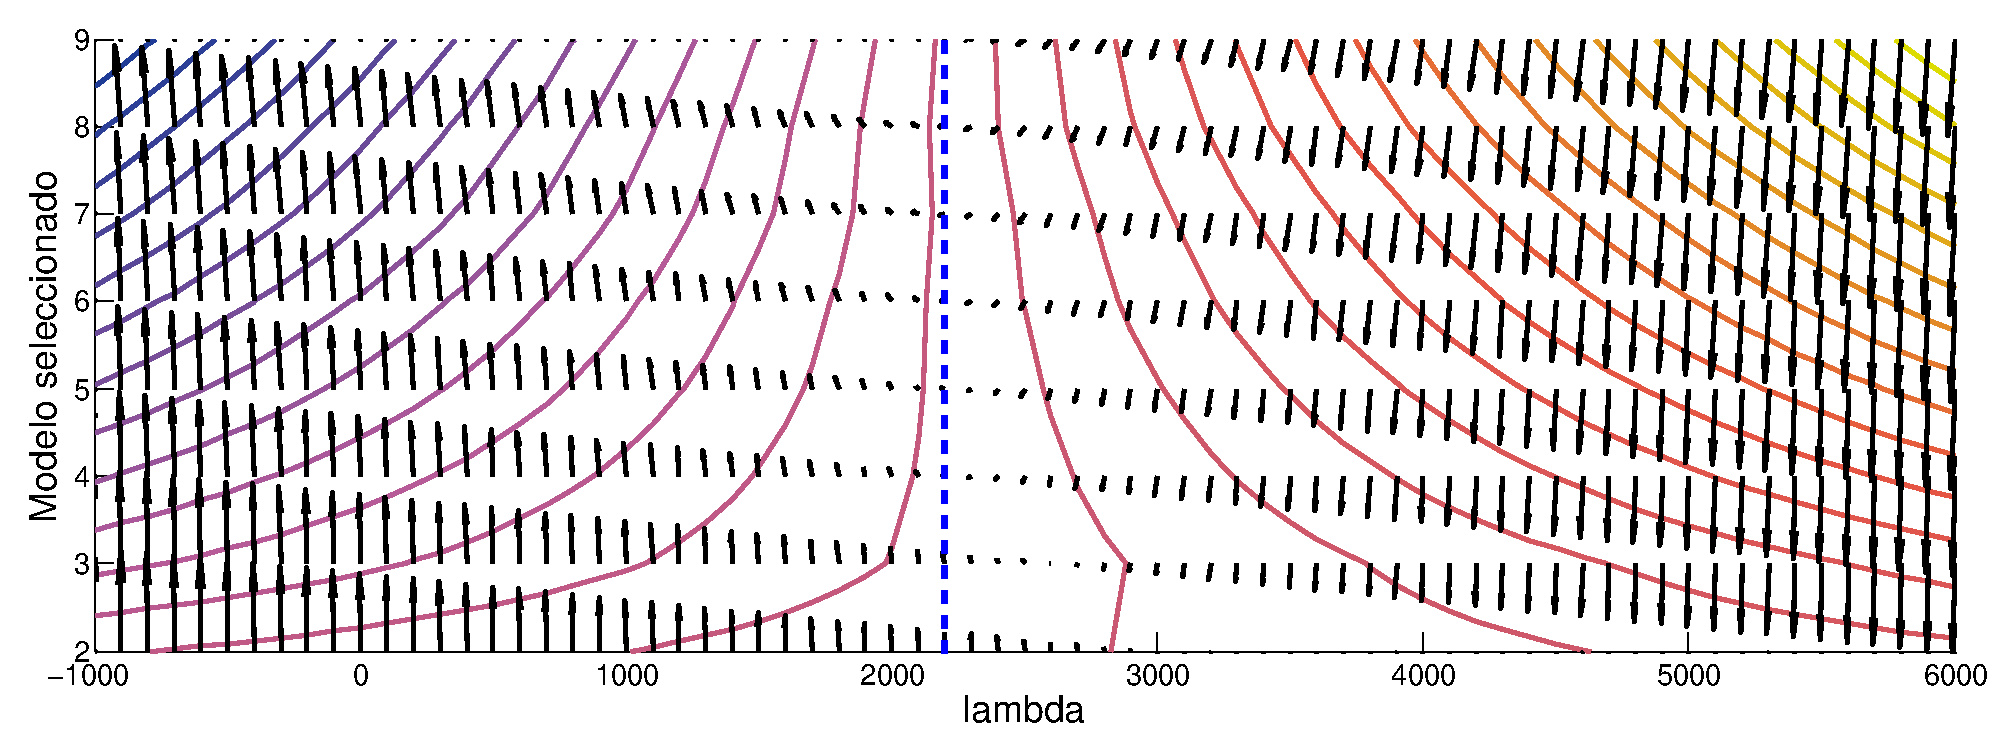
\includegraphics[width=1\textwidth]{gfx/chap6/lear3bic2}
   \caption{}
   \label{fig:seq3_bic2}
  \end{subfigure}  
  }  
  \centerline{
  \begin{subfigure}[b]{0.4\textwidth}
    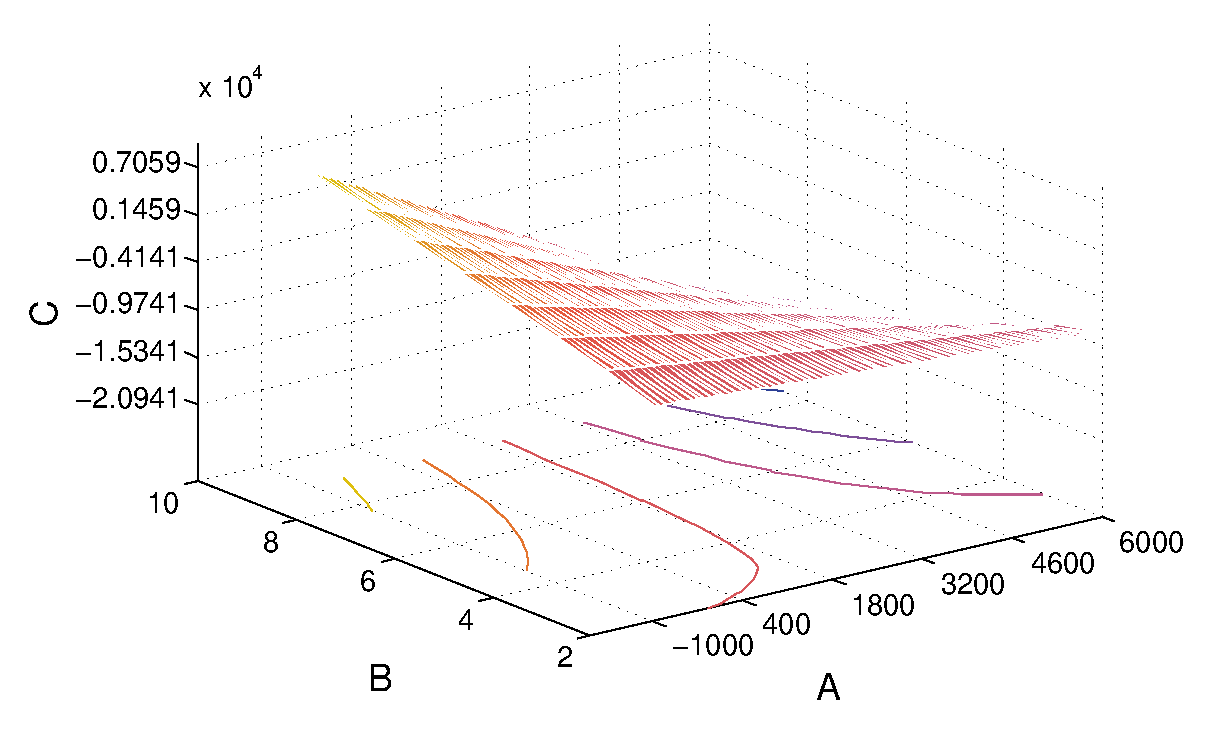
\includegraphics[width=\textwidth]{gfx/chap6/lear3bic1} 
    \caption{}
    \label{fig:seq3_bic1}
  \end{subfigure}  
  \begin{subfigure}[b]{0.4\textwidth}
    \includegraphics[width=\textwidth]{gfx/chap6/lear3bic3} 
    \caption{}
    \label{fig:seq3_bic3}
  \end{subfigure}
  }
  \label{fig:seq1_bic}
\end{figure}
\end{frame}

\begin{frame}{Secuencia 3}{Pruebas de hipótesis}
\begin{figure}[t!]
  \centerline  
  { \begin{subfigure}[b]{0.45\textwidth}
      \includegraphics[width=1\linewidth]{gfx/chap6/lear3boot1}
      \caption{}
      \label{fig:seq3_boot1}
    \end{subfigure}
    \hspace{0.5cm}
    \begin{subfigure}[b]{0.45\textwidth}
      \includegraphics[width=1\linewidth]{gfx/chap6/lear3boot2}
      \caption{}
      \label{fig:seq3_boot2}
    \end{subfigure}
  }
  \centerline  
  { \begin{subfigure}[b]{0.45\textwidth}
      \includegraphics[width=1\linewidth]{gfx/chap6/lear3boot3}
      \caption{}
      \label{fig:seq3_boot3}
    \end{subfigure}
    \hspace{0.5cm}
    \begin{subfigure}[b]{0.45\textwidth}
      \includegraphics[width=1\linewidth]{gfx/chap6/lear3boot4}
      \caption{}
      \label{fig:seq3_boot4}
    \end{subfigure}
  }
  \label{fig:seq3_boot}
\end{figure}
\end{frame}

\begin{frame}{Secuencia 3}{Secuencia recuperada}
\begin{figure}[tp]
  \centerline
  {\begin{subfigure}[b]{0.8\textwidth}
      \includegraphics[width=1\linewidth]{gfx/chap6/lear3s_3_1}
      \caption{}
      \label{fig:seq3_seq1}
    \end{subfigure}
  } 
  \centerline
  {\begin{subfigure}[b]{0.8\textwidth}
      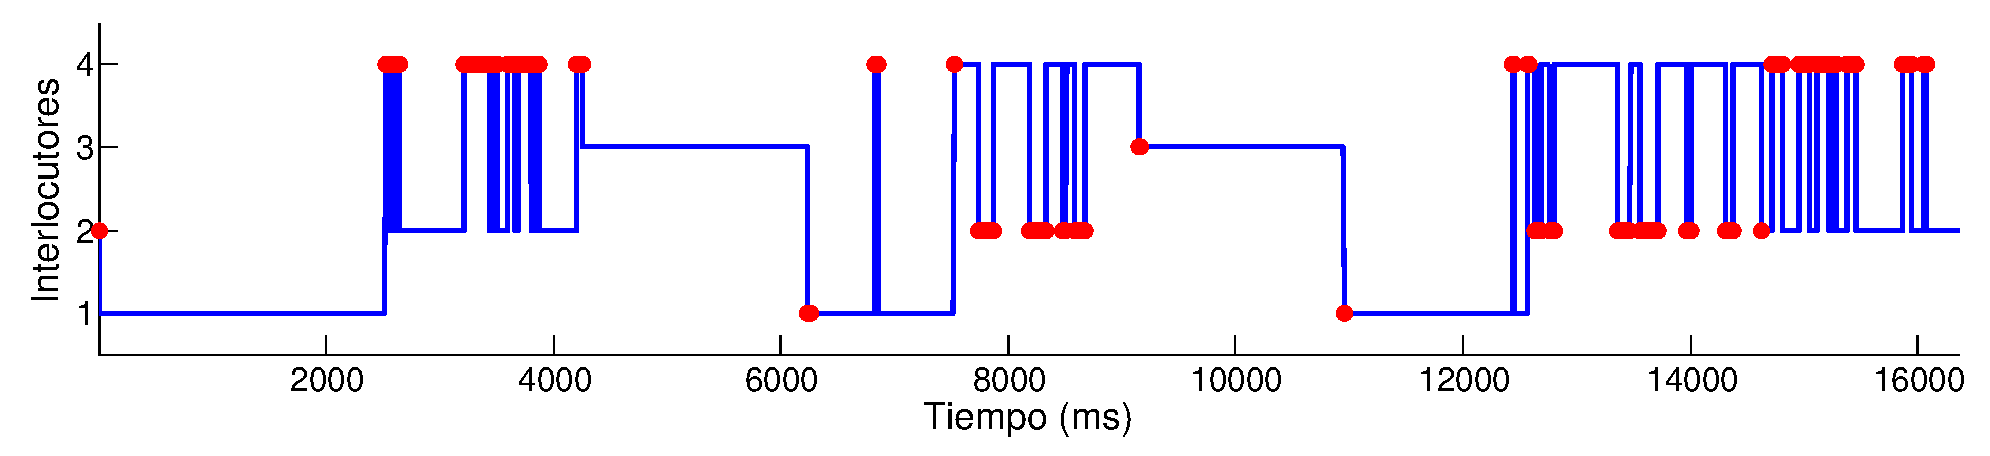
\includegraphics[width=1\linewidth]{gfx/chap6/lear3s_3_2}
      \caption{}
      \label{fig:seq3_seq2}
    \end{subfigure}
  }
  \label{fig:prb3_seq}
\end{figure}
\end{frame}

\subsection{Resultados}
\begin{frame}{Tabla de resultados (I)}
  Descripción de las secuencias de audio utilizadas para las pruebas.
  \begin{figure}[bth]
    \centerline
    {\includegraphics[width=0.7\linewidth]{gfx/tab1}}
    \label{fig:esquema}
  \end{figure}  
\end{frame}

\begin{frame}{Tabla de resultados (II)}
  Detalle de los resultados para todas las secuencias de audio.
  \begin{figure}[bth]
    \centerline
    {\includegraphics[width=0.7\linewidth]{gfx/tab2}}
    \label{fig:esquema}
  \end{figure}  
\end{frame}